\section{Lösungsansatz 1 S}

Zur Berechnung größerer Graphen gibt es sogenannten metaheuristische Verfahren die keine optimale Lösung garantieren.
Durch probabilistische Schätzungen und heuristische Verfahren können jedoch gute Lösungen gefunden werden.
\\\\
Eines dieser metaheuristischen Verfahren ist der Ant Algorithm (auch \glqq Ant Colony Optimization\grqq{} oder \glqq \acs{aco}\grqq{} genannt).
Dies ist ein Algorithmus der sich an dem Verhalten von Schwärmen von Tieren orientiert.
Ein Schwarm besteht aus einer Gruppe von \glqq Agenten\grqq{} die miteinander kommunizieren, um eine Lösung zu finden.
Der \acs{aco} basiert auf dem Verhalten von Ameisen, die Pfade zu Nahrungsquellen aufspüren.
\\
Der Algorithmus simuliert die Aktivitäten von Ameisen, die zufällig durch die Städte wandern und dabei Informationen über die Qualität der verschiedenen möglichen Pfade sammeln.
Bei jeder Bewegung einer Ameise werden auf dem gewählten Pfad Pheromone (Duftstoffe) hinterlassen.
Diese Informationen werden dann verwendet, um die Wahrscheinlichkeit zu bestimmen, dass eine bestimmte Ameise einen bestimmten Pfad wählt, wenn sie von einer Stadt zu einer anderen reist. 
\\
Zur weiteren Optimierung der Tour werden nacheinander mehrere Generationen von Schwärmen durchlaufen.
Jede Generation bekommt die Wahrscheinlichkeiten der Pfade der vorherigen Generation und baut darauf auf.
Auf diese Weise kann der Algorithmus schrittweise die optimale Tour durch die Städte bestimmen.

\begin{figure}[H]
    \centering
    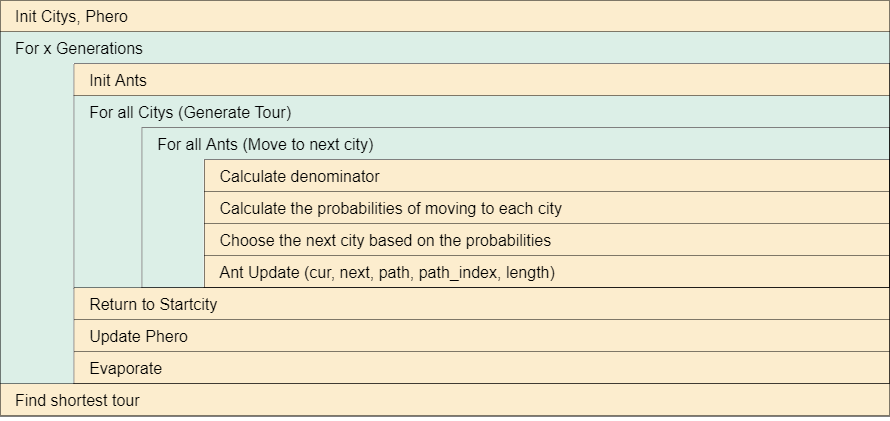
\includegraphics[width=16cm]{../images/struktog.png}
    \caption{Algorithmus Struktogramm}
    \label{fig:struktogramm}
\end{figure}

\section{Implementierung inklusive Schwierigkeiten}
1 - 2 Seiten

\section{Bewertung}
Bewertung des Ansatzes und der performance-limitierenden Faktoren (1-2 Seiten)
